\documentclass[12pt,aspectratio=169]{beamer}
\usetheme{aurigapolimi}

\setbeamertemplate{bibliography item}{\insertbiblabel}

% % % % PACKAGES % % % % % % % % % % % % %
\usepackage{booktabs}
\usepackage{amsmath,amssymb}
\usepackage{tikz}
\usetikzlibrary{positioning}
\usepackage[ruled,vlined,linesnumbered]{algorithm2e}
\graphicspath{{figures/}}

% = = = = = = = = = = = = = = = = = = = =
% Algorithm environment styling
% = = = = = = = = = = = = = = = = = = = =
\DontPrintSemicolon
\SetAlgoCaptionSeparator{:}
% drop the algorithm number: caption reads "Algorithm: UCB1"
\renewcommand{\thealgocf}{\kern-0.35em}
\SetAlCapNameFnt{\normalfont}
\SetAlCapFnt{\normalfont}
\SetAlgoInsideSkip{smallskip}

% light-blue panel behind each algorithm box
\definecolor{algobg}{RGB}{223,238,250}
\setbeamercolor{algobox}{bg=algobg,fg=black}
\newenvironment{algobox}[1][\textwidth]
  {\begin{beamercolorbox}[sep=0.45em,wd=#1]{algobox}}
  {\end{beamercolorbox}}

% % % % METADATA % % % % % % % % % % % %

\title{Online Learning Applications}
\subtitle{Multiple advertising campaigns under budget constraints}
\author{
  Name - ID,
  Name - ID,\\
  Sergio Ligregni - 11151186,
  Anh Chi Tuan - 11056931}

\institute{September 8\textsuperscript{\tiny{th}}, 2026 }
\setaurigadate{}
\selectcolor{deepBluePolimi} % lighter polimi blue also available (bluePolimi)


% = = = = = = = = = = = = = = = = = = = =
% Set up logos = = = = = = = = = = = = =
% = = = = = = = = = = = = = = = = = = = =

% Title-page logos
\setaurigatitlelogoA{logos/polimi_logo.eps}
\setaurigatitlelogoheightA{1.5cm}

%\setaurigatitlelogoB{logos/uab_text.eps}
%\setaurigatitlelogoheightB{1.8cm}

% Slide logos
\setaurigalogoA{logos/polimi_logo.eps}
\setaurigalogoheightA{0.5cm}

%\setaurigalogoB{logos/}
\setaurigalogoheightB{}

\begin{document}
\aurigatitleframe

\newcommand{\iid}{\stackrel{\tiny{iid}}{\sim}}
\newcommand{\ind}{\stackrel{\tiny{ind}}{\sim}}

% = = = = = = = = = = = = = = = = = = = =
% Handy shorthands for the deck
% = = = = = = = = = = = = = = = = = = = =
\newcommand{\bidset}{\mathcal{B}}
\newcommand{\campaigns}{\mathcal{N}}
\newcommand{\superarms}{\mathcal{S}}
\newcommand{\OPT}{\mathrm{OPT}}
\newcommand{\ucb}{\widehat{f}^{\,\mathrm{UCB}}}
\newcommand{\lcb}{\widehat{c}^{\,\mathrm{LCB}}}

% Placeholder boxes: delete once the real figures exist
% \figph[width]{caption}   \figphx{width}{height}{caption}
\newcommand{\figphx}[3]{%
  \fbox{\parbox[c][#2][c]{#1}{\centering\ttfamily\small #3}}}
\newcommand{\figph}[2][0.8\textwidth]{\figphx{#1}{3.2cm}{#2}}


% = = = = = = = = = = = = = = = = = = = =
\begin{frame}{Outline}
  \tableofcontents
\end{frame}
% = = = = = = = = = = = = = = = = = = = =


% ####################################################################
\section{Problem setting}
% ####################################################################

\begin{frame}{The problem}
\footnotesize
  \textbf{An advertiser bids in repeated first-price auctions across several campaigns, spending one shared budget.}
  \begin{itemize}
    \item $T$ rounds, $N$ campaigns, discrete bid set $\bidset$.
    \item Each round: pick a set of campaigns and a bid for each; win campaign $i$ iff
          $b_i \ge m_i$ (highest competing bid).
    \item Utility $v_i - b_i$ on a win, cost $b_i$; total spend $\le B$.
    \item A \emph{conflict graph} forbids some campaigns from running in the same round.
  \end{itemize}
  \begin{block}{Goal}
    Minimise regret w.r.t.\ the best budget-feasible benchmark.
  \end{block}
\end{frame}

\begin{frame}{Environment}
\scriptsize
\textbf{How the competition is simulated.}
Campaign $i$ has $k_i$ competitors, each bidding $\mathrm{U}[0,1]$ independently.
Only the \emph{highest} competing bid matters, and the max of $k_i$ uniforms is a Beta:
\[
  m_i(t)=\max_{j\le k_i} u_j\sim\mathrm{Beta}(k_i,1)
  \quad\Longrightarrow\quad
  \mathbb{P}(b\ge m_i)=F_{\mathrm{Beta}(k_i,1)}(b)=b^{\,k_i}.
\]
More competitors $\Rightarrow$ steeper curve, you must bid higher to win.
We only allow bids $b\le v_i$ (bidding above the valuation never gives positive utility).
\vspace{0.1cm}
\begin{center}
  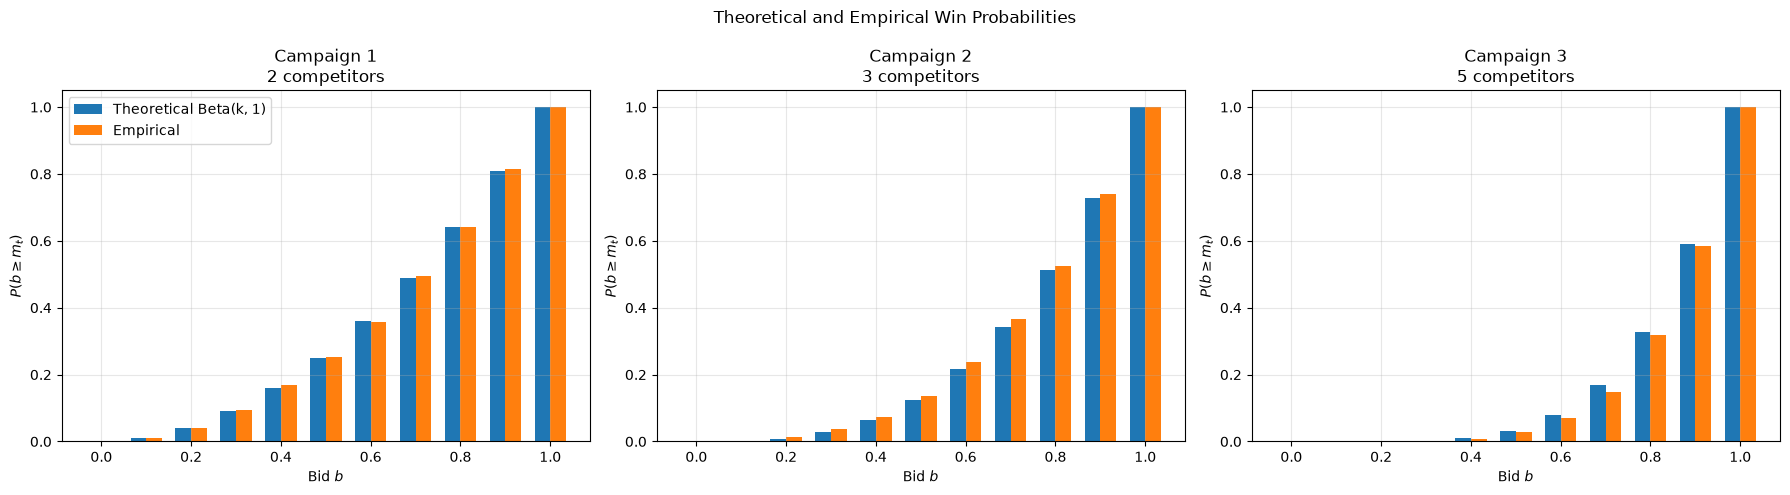
\includegraphics[width=0.95\textwidth,height=0.42\textheight,keepaspectratio]{req2_estimation.png}\\[-0.05cm]
  {\tiny Theoretical $b^{k_i}$ vs.\ empirical win frequency over $T{=}2000$ rounds, $k=(2,3,5)$.
  All requirements share this generator; R3/R4 let $k_i$ change over time.}
\end{center}
\end{frame}

\begin{frame}{Conflict graph}
\scriptsize
\begin{columns}[T]
  \begin{column}{0.55\textwidth}
    \textbf{Some campaigns cannot run together} (e.g.\ two direct competitors).
    \begin{itemize}
      \item Nodes = campaigns, edge = ``mutually exclusive''.
            Here campaigns 2 and 3 conflict; campaign 1 is compatible with both.
      \item Per round we may only activate an \emph{independent set}:
            $\emptyset,\{1\},\{2\},\{3\},\{1,2\},\{1,3\}$.
      \item An action is a \textbf{super-arm} $a=(S,b_S)$: a feasible set $S$ plus one bid per
            campaign in $S$. With $b\le v_i$ this gives $|\mathcal A|=102$ super-arms.
      \item Consequence: campaigns cannot be optimised independently any more,
            \emph{which} campaigns to run is part of the decision.
    \end{itemize}
  \end{column}
  \begin{column}{0.42\textwidth}
    \centering
    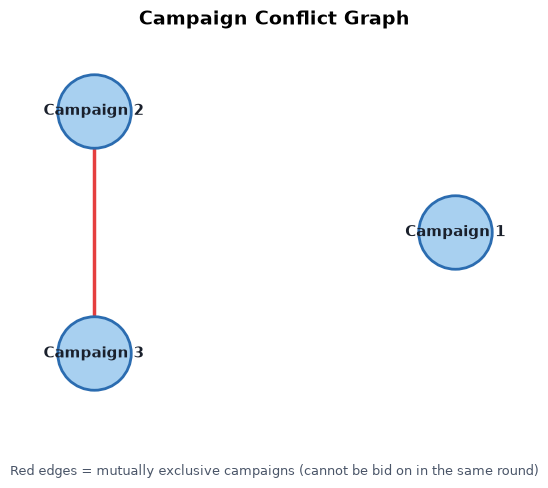
\includegraphics[width=\linewidth,height=0.6\textheight,keepaspectratio]{req2_conflict_graph.png}
  \end{column}
\end{columns}
\end{frame}

% ####################################################################
\section{Requirement 1 --- Single campaign, stochastic}
% ####################################################################

\begin{frame}{R1 --- Environment setting}
\scriptsize
\begin{columns}[T]
  \begin{column}{0.55\textwidth}
    \textbf{One campaign, stochastic competitors.}
    \begin{itemize}
      \item $k=3$ competitors with $\mathrm{U}[0,1]$ bids
            $\Rightarrow m_t\sim\mathrm{Beta}(3,1)$, i.i.d.\ over rounds.
      \item Valuation $v=0.6$, horizon $T=5000$, budget $B=300$
            ($\rho=B/T=0.06$ per round).
      \item Bid set $\bidset=\{0,0.1,\dots,1\}$ restricted to $b\le v$ $\Rightarrow$ 6 arms.
      \item Reward and cost of bid $b$ at round $t$:
            \[ f_t(b)=(v-b)\,\mathbb 1\{b\ge m_t\},\qquad c_t(b)=b\,\mathbb 1\{b\ge m_t\}. \]
      \item Bandit feedback: we only see whether \emph{our} bid won.
    \end{itemize}
  \end{column}
  \begin{column}{0.43\textwidth}
    \centering
    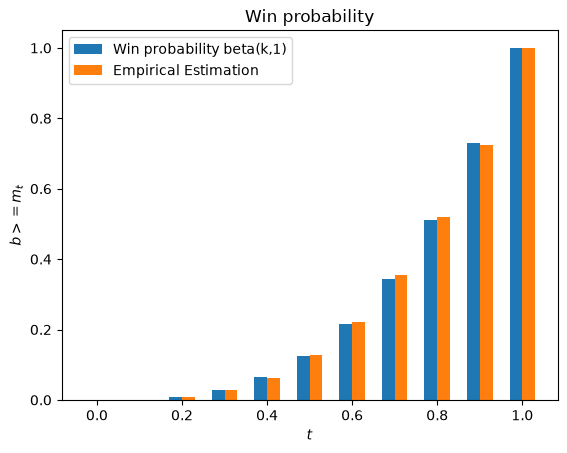
\includegraphics[width=\linewidth,height=0.58\textheight,keepaspectratio]{req1_estimation.png}\\[0.03cm]
    {\tiny Win probability $b^{3}$ (blue) vs.\ empirical frequency over $5000$ rounds (orange).}
  \end{column}
\end{columns}
\end{frame}

\begin{frame}{R1 --- Baseline (Clairvoyant)}
\scriptsize
\begin{columns}[T]
  \begin{column}{0.55\textwidth}
    \textbf{Without budget.} Expected reward of a bid is $\mu(b)=(v-b)\,b^{k}$, so
    \[ b^\star=\tfrac{k}{k+1}\,v = 0.45 \;\Rightarrow\; \text{closest arm } 0.4,\quad \mu(0.4)=0.0128 . \]
    \textbf{With budget.} The clairvoyant knows the distribution (not the realisations) and solves
    \[
      \max_{\gamma\in\Delta(\bidset)}\;\sum_b \gamma(b)(v-b)\,b^{k}
      \quad\text{s.t.}\quad \sum_b \gamma(b)\,b\,b^{k}\le\rho .
    \]
    Here $\rho=0.06$ but the best arm costs only $0.4\cdot0.4^3=0.026$ per round:
    the budget is \emph{not binding}, $\gamma^\star=\delta_{0.4}$ and both baselines
    coincide, $\OPT=0.0128$ per round.
  \end{column}
  \begin{column}{0.43\textwidth}
    \centering
    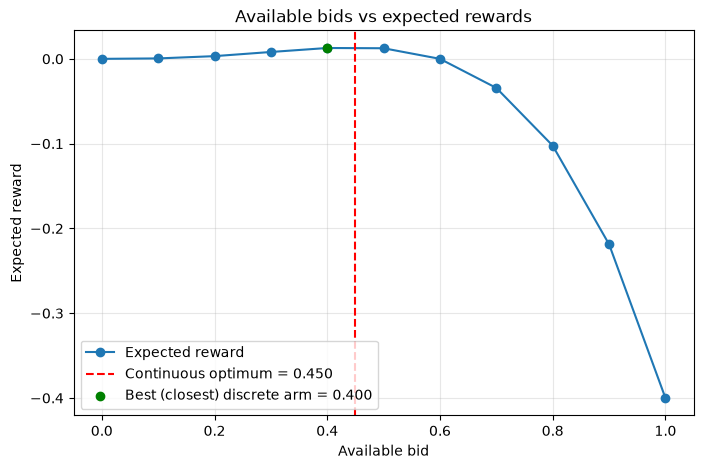
\includegraphics[width=\linewidth,height=0.58\textheight,keepaspectratio]{r1_expected_reward.png}\\[0.03cm]
    {\tiny $\mu(b)$ over the arms; $0.4$ and $0.5$ are almost equally good.}
  \end{column}
\end{columns}
\end{frame}
% - - - - - - - - - - - - - - - - - - - -
\begin{frame}{R1 --- Algorithm (i): UCB1, without budget constraint}
  \begin{algobox}
  \begin{algorithm}[H]
    \footnotesize
    \caption{UCB1 for single campaign without budget constraint}
    \KwIn{set of arms $A$, number of rounds $T$, valuation $v$}
    \For{$t = 1,\dots,T$}{
      \ForEach{$a \in A$}{
        $\mu_t(a) \leftarrow \dfrac{1}{N_{t-1}(a)}\sum_{t'=1}^{t-1} r_{t'}(a)\,
          \mathbb{I}[a_{t'} = a]$\;
        $UCB_t(a) \leftarrow \mu_t(a) + v\sqrt{\dfrac{2\log T}{N_{t-1}(a)}}$\;
      }
      play $a_t \in \arg\max_a UCB_t(a)$; observe $r_t$ and update $N_t,\mu_t$\;
    }
  \end{algorithm}
  \end{algobox}
  \vspace{0.1cm}
  \scriptsize
  Plain UCB1: rewards live in $[0,v]$ so the bonus is scaled by $v$; try every arm once,
  then be optimistic. The budget is simply ignored.
\end{frame}

% - - - - - - - - - - - - - - - - - - - -
\begin{frame}{R1 --- Algorithm (ii): UCB1 under the budget}

  \begin{algobox}
  \begin{algorithm}[H]
    \scriptsize
    \caption{\scriptsize UCB1 for single campaign with budget constraint}
    \KwIn{bid set $\bidset$, number of rounds $T$, budget $B$, value $v$}
    \For{$t = 1,\dots,T$}{
      \ForEach{$b \in \bidset$}{
        $\overline{f}_t(b)\leftarrow\frac{1}{N_{t-1}(b)}\sum_{t'=1}^{t-1}f_{t'}(b)\mathbb{I}(b_{t'}=b)$\;
        $\overline{f}_t^{UCB}(b)\leftarrow\overline{f}_t(b)+v\sqrt{\frac{2\log(T)}{N_{t-1}(b)}}$\;
        $\overline{c}_t(b)\leftarrow\frac{1}{N_{t-1}(b)}\sum_{t'=1}^{t-1}c_{t'}(b)\mathbb{I}(b_{t'}=b)$\;
        $\overline{c}_t^{LCB}(b)\leftarrow\overline{c}_t(b)-v\sqrt{\frac{2\log(T)}{N_{t-1}(b)}}$\;
      }
      $\gamma_t\leftarrow\arg\max_{\gamma\in\Delta(\bidset)}\sum_b\gamma(b)\overline{f}_t^{UCB}(b)$
      s.t. $\sum_b\gamma(b)\overline{c}_t^{LCB}(b)\le\rho$\;
      Bid $b_t \sim \gamma_t$; observe $f_t(b_t)$, $c_t(b_t)$; $B\leftarrow B-c_t(b_t)$\;
      \lIf{$B<1$}{Terminate}
    }
  \end{algorithm}
  \end{algobox}
\end{frame}

\begin{frame}{R1 --- Results}
\scriptsize
\begin{columns}[T]
  \begin{column}{0.5\textwidth}
    \centering
    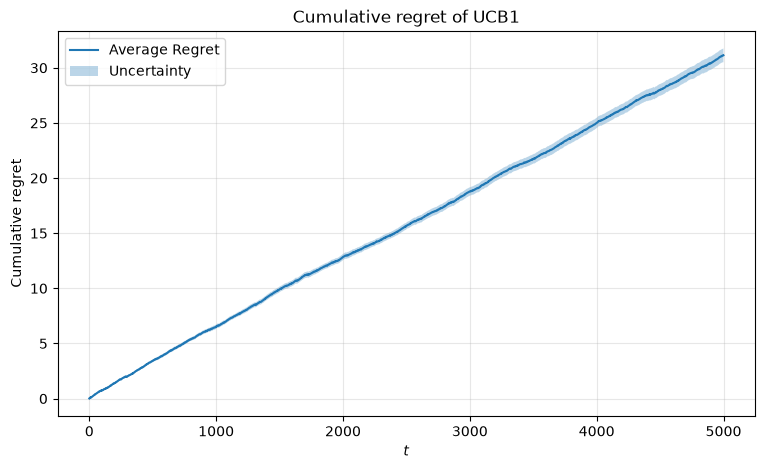
\includegraphics[width=\linewidth,height=0.42\textheight,keepaspectratio]{r1_ucb1_regret.png}\\[0.02cm]
    {\tiny (i) UCB1 without budget, 30 trials. Final regret $\approx 31$.}
  \end{column}
  \begin{column}{0.5\textwidth}
    \centering
    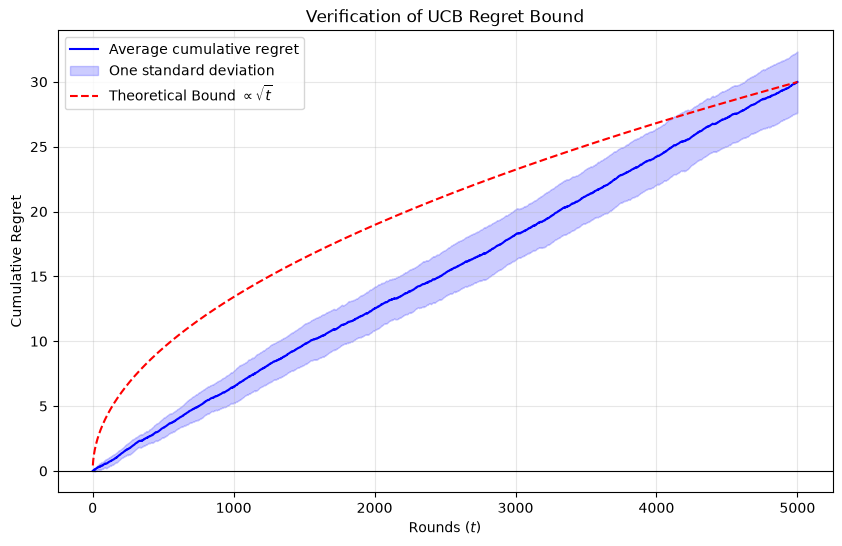
\includegraphics[width=\linewidth,height=0.42\textheight,keepaspectratio]{r1_budget_regret.png}\\[0.02cm]
    {\tiny (ii) UCB-like with budget, 30 trials, with a $\propto\!\sqrt t$ reference. Final regret $\approx 30$.}
  \end{column}
\end{columns}
\vspace{0.1cm}
\begin{itemize}
  \item Both learners concentrate on arms $0.4$ and $0.5$ ($\sim\!950$ pulls each). Their gap is
        only $3\cdot10^{-4}$, far below the confidence radius, so they are hard to tell apart and
        the regret keeps growing slowly ($\approx 0.006$ per round).
  \item The budget is never exhausted (spend $\approx 85$ of $300$, see appendix), so (i) and (ii)
        behave alike here; the LP only matters when $\rho$ is binding.
\end{itemize}
\end{frame}



% ####################################################################
\section{Requirement 2 --- Multiple campaigns, stochastic}
% ####################################################################

\begin{frame}{R2 --- Environment setting}
\scriptsize
\textbf{$N=3$ campaigns, one shared budget.}
\begin{itemize}
  \item Valuations $v=(0.4,0.6,0.8)$, competitors $k=(2,3,5)$
        $\Rightarrow m_i(t)\sim\mathrm{Beta}(k_i,1)$ independently per campaign.
  \item $T=2000$, $B=100$ $\Rightarrow$ $\rho=0.05$ per round (now \emph{binding}).
        Bid set $\{0,0.1,\dots,1\}$ with $b\le v_i$; campaigns 2 and 3 mutually exclusive.
  \item Per round we play a super-arm $a=(S,b_S)$ and collect
        $f_t(a)=\sum_{i\in S}(v_i-b_i)\mathbb 1\{b_i\ge m_i(t)\}$,
        $c_t(a)=\sum_{i\in S} b_i\,\mathbb 1\{b_i\ge m_i(t)\}$.
  \item Semi-bandit feedback: we observe win/loss for every campaign we bid on.
\end{itemize}
\begin{center}
  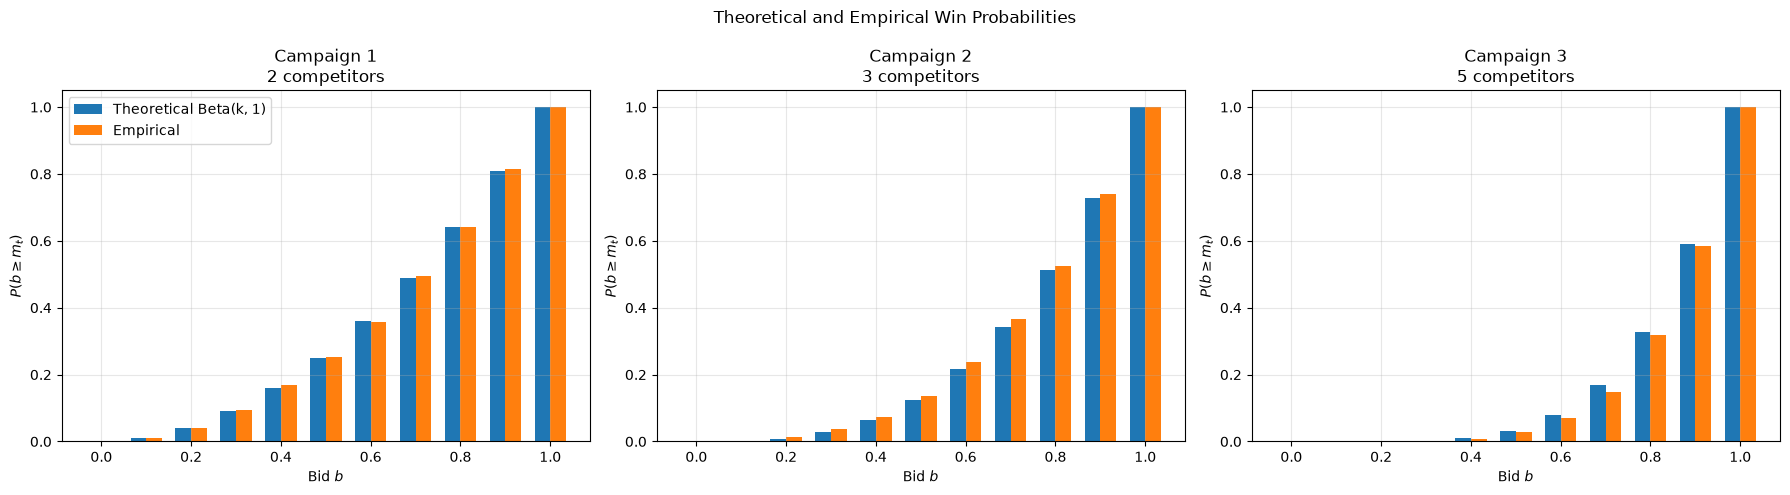
\includegraphics[width=0.95\textwidth,height=0.4\textheight,keepaspectratio]{req2_estimation.png}\\[-0.05cm]
  {\tiny Campaign 3 pays a lot more to win: 5 competitors, $\mathbb P(\text{win})=b^5$.}
\end{center}
\end{frame}

\begin{frame}{R2 --- Baseline (Clairvoyant)}
\scriptsize
\textbf{One LP over super-arms} (expected values, budget only in expectation):
\[
  \max_{\gamma\in\Delta(\mathcal A)}\;\sum_{a\in\mathcal A}\gamma(a)\,\bar f(a)
  \quad\text{s.t.}\quad \sum_{a\in\mathcal A}\gamma(a)\,\bar c(a)\le\rho,
  \qquad
  \bar f(a)=\sum_{i\in S}(v_i-b_i)\,b_i^{k_i},\;\;
  \bar c(a)=\sum_{i\in S} b_i\,b_i^{k_i}.
\]
\begin{columns}[T]
  \begin{column}{0.5\textwidth}
    \textbf{Without conflict graph} (3 independent simplices):
    \begin{center}\scriptsize
    \begin{tabular}{@{}lll@{}}
      \toprule
      Campaign & Bid & Prob.\\
      \midrule
      1 & $0.2$ & $1$\\
      2 & $0.4$ & $1$\\
      3 & $0.5$ / $0.6$ & $0.975$ / $0.025$\\
      \bottomrule
    \end{tabular}
    \end{center}
    $\OPT=0.0303$ per round, spends exactly $\rho=0.05$.
  \end{column}
  \begin{column}{0.5\textwidth}
    \textbf{With conflict graph} (102 super-arms, 2 and 3 exclusive):
    \begin{center}\scriptsize
    \begin{tabular}{@{}lll@{}}
      \toprule
      Super-arm & Bids & Prob.\\
      \midrule
      $S=\{1,2\}$ & $(0.2,\,0.4)$ & $0.22$\\
      $S=\{1,3\}$ & $(0.2,\,0.6)$ & $0.78$\\
      \bottomrule
    \end{tabular}
    \end{center}
    $\OPT=0.0229$ per round, spends exactly $\rho=0.05$.\\[0.1cm]
    The budget is tight, so the optimum \emph{mixes} two super-arms; the conflict costs
    about a quarter of the reward.
  \end{column}
\end{columns}
\end{frame}
% - - - - - - - - - - - - - - - - - - - -
\begin{frame}{R2 --- Algorithm: Combinatorial UCB with budget}
\scriptsize
\textbf{Idea.} Keep UCB statistics on the \emph{base arms} (campaign, bid), combine them into
optimistic values of every super-arm, and solve the clairvoyant LP with those values.
\begin{algobox}
\begin{algorithm}[H]
  \scriptsize
  \caption{\scriptsize Combinatorial-UCB for multiple campaigns with budget}
  \KwIn{super-arms $\mathcal A$, $T$, $B$, valuations $v$;\; $\rho\leftarrow B/T$, all base-arm statistics $N,\bar f,\bar c\leftarrow0$}
  \For{$t=1,\dots,T$}{
    \lIf{$B<1$}{play $(\emptyset,\emptyset)$ and continue}
    \ForEach{base arm $(i,b)$}{
      $\ucb(i,b)\leftarrow \bar f(i,b)+v_i\sqrt{2\log T/N(i,b)}$
      \quad ($=+\infty$ if $N(i,b)=0$)\;
      $\lcb(i,b)\leftarrow \max\{0,\;\bar c(i,b)-v_i\sqrt{2\log T/N(i,b)}\}$\;
    }
    \lForEach{super-arm $a=(S,b_S)$}{
      $\ucb(a)\leftarrow\sum_{i\in S}\ucb(i,b_i)$,\;
      $\lcb(a)\leftarrow\sum_{i\in S}\lcb(i,b_i)$}
    $\gamma_t\leftarrow\arg\max_{\gamma\in\Delta(\mathcal A)}\sum_a\gamma(a)\ucb(a)$
      s.t. $\sum_a\gamma(a)\lcb(a)\le\rho$\;
    sample $a_t\sim\gamma_t$, bid on $S_t$, observe $f_t(i,b_i),c_t(i,b_i)$ for each $i\in S_t$\;
    update $N,\bar f,\bar c$ of the played base arms;\; $B\leftarrow B-c_t(a_t)$\;
  }
\end{algorithm}
\end{algobox}
\end{frame}

% - - - - - - - - - - - - - - - - - - - -
\begin{frame}{R2 --- Why base arms instead of super-arms}
\scriptsize
\begin{columns}[T]
  \begin{column}{0.6\textwidth}
    \begin{itemize}
      \item Treating the $102$ super-arms as independent arms would need $\sim\!100$ rounds just
            to try each once, and nothing learned on one would help the others.
      \item The reward of a super-arm is \emph{additive} over its campaigns, so we estimate the
            base arms $(i,b)$ and sum them: one round on $\{1,3\}$ improves \emph{every}
            super-arm containing $(1,0.3)$ or $(3,0.7)$.
      \item Confidence radius scaled by $v_i$ because rewards live in $[0,v_i]$.
      \item Unexplored base arms get an optimistic placeholder (huge UCB, zero LCB) so they are
            tried first.
      \item The LP over super-arms already encodes the conflict graph: infeasible sets are
            simply not in $\mathcal A$.
    \end{itemize}
  \end{column}
  \begin{column}{0.38\textwidth}
    \centering
    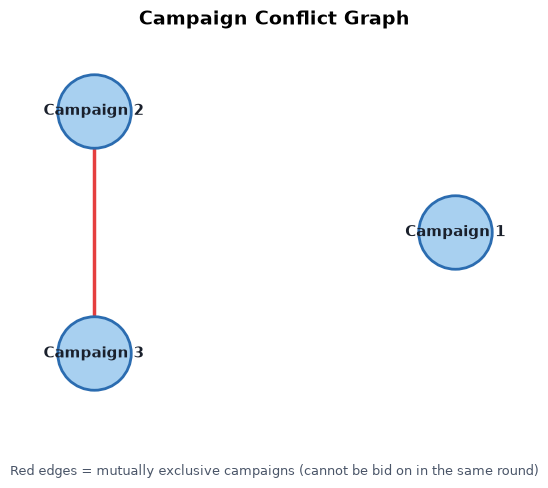
\includegraphics[width=\linewidth,height=0.55\textheight,keepaspectratio]{req2_conflict_graph.png}
  \end{column}
\end{columns}
\end{frame}

\begin{frame}{R2 --- Results}
\scriptsize
\begin{columns}[T]
  \begin{column}{0.5\textwidth}
    \centering
    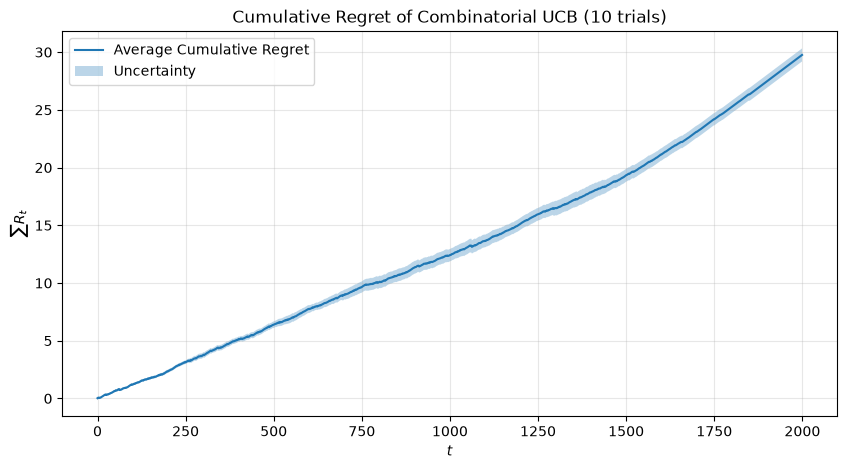
\includegraphics[width=\linewidth,height=0.42\textheight,keepaspectratio]{req2_cumregret.png}\\[0.02cm]
    {\tiny Cumulative regret, 10 trials ($T\cdot\OPT=45.9$).}
  \end{column}
  \begin{column}{0.5\textwidth}
    \centering
    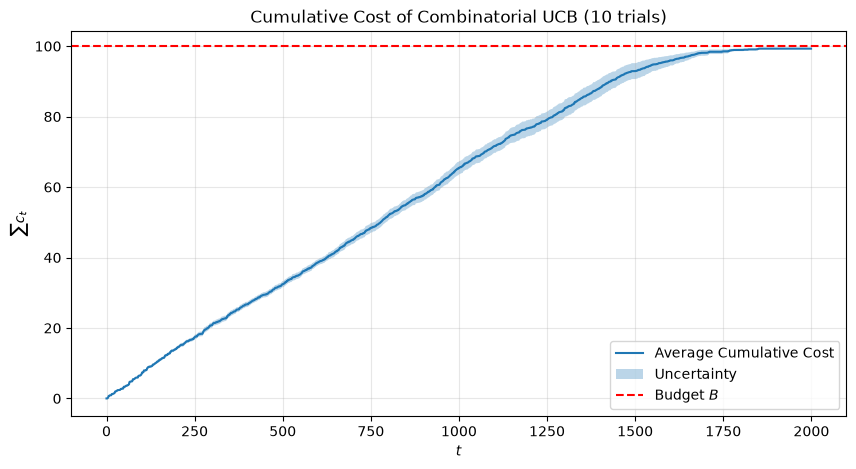
\includegraphics[width=\linewidth,height=0.42\textheight,keepaspectratio]{req2_cum_cost.png}\\[0.02cm]
    {\tiny Cumulative cost vs.\ budget $B=100$.}
  \end{column}
\end{columns}
\vspace{0.1cm}
\begin{itemize}
  \item Final regret $\approx 30$ against $\OPT$ with conflict graph; the budget is never violated
        (spent $99.3$ of $100$).
  \item Up to $t\approx1500$ the regret grows slowly: the learner finds the right super-arms.
        Optimistic (low) cost estimates then make it spend slightly faster than $\rho$, the budget
        runs out around $t\approx1700$, and from there it must play $(\emptyset,\emptyset)$,
        so the regret bends upward at rate $\OPT$ per round.
  \item Pacing the spend evenly over the horizon is exactly what the primal-dual method of R3 adds.
\end{itemize}
\end{frame}

% ####################################################################
\section{Requirement 3 --- Best of both worlds}
% ####################################################################

\begin{frame}{R3 --- Environment setting}
\scriptsize
\begin{columns}[T]
  \begin{column}{0.47\textwidth}
    \textbf{Two environments from one generator.}
    \begin{itemize}
      \item \textbf{Stationary (R2):} fixed competitors $k=(2,3,5)$,
            so $m_i(t)\sim\mathrm{Beta}(k_i,1)$.
      \item \textbf{Non-stationary:} $k_i(t)$ cycles through $\kappa_i$ every $L_i$
            rounds, unsynchronised across campaigns:
            $\kappa_1{=}(1,3),\,L_1{=}10$;\;
            $\kappa_2{=}(1,5,3),\,L_2{=}20$;\;
            $\kappa_3{=}(6,1,3),\,L_3{=}30$.
      \item Win probability $b^{\,k_i(t)}$ changes every few rounds, so the optimal
            bid and budget allocation change over time.
      \item One fixed seeded sequence (oblivious adversary).
    \end{itemize}
    \vspace{0.05cm}
    {\tiny $T{=}2000$, $N{=}3$, $v{=}(0.6,0.7,0.8)$, $B{=}300$ ($\rho{=}0.15$);
    campaigns 2--3 mutually exclusive.}
  \end{column}
  \begin{column}{0.50\textwidth}
    \centering
    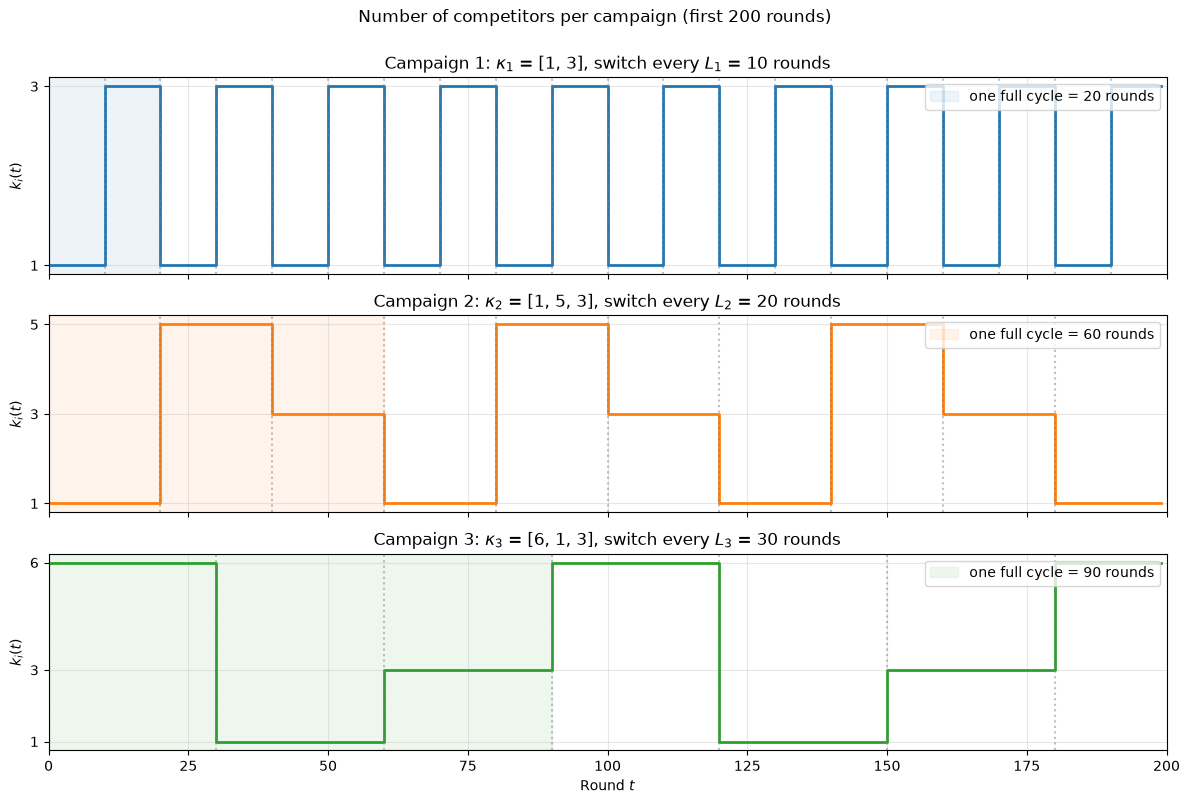
\includegraphics[width=\linewidth,height=0.52\textheight,keepaspectratio]{r3_k_schedule.png}\\[0.05cm]
    {\tiny $k_i(t)$: regimes switch every $L_i$ rounds (first 200 rounds).}
  \end{column}
\end{columns}
\end{frame}

\begin{frame}{R3 --- Baseline: best strategy in hindsight}
\scriptsize
\begin{columns}[T]
  \begin{column}{0.51\textwidth}
    Non-stochastic $\Rightarrow$ benchmark: best \emph{fixed} super-arm distribution
    on the realised sequence, under budget and conflict graph:
    $\OPT=\max_{\gamma\in\Delta_{\mathcal A}}\sum_{t=1}^{T} f_t(\gamma)$
    subject to $\sum_{t=1}^{T} c_t(\gamma)\le B,$
    where $f_t(\gamma)=\sum_{a}\gamma(a)f_t(a)$,
    $c_t(\gamma)=\sum_{a}\gamma(a)c_t(a)$, and
    \begin{align*}
      f_t(a)&=\sum_{i\in S}(v_i-b_i)\,\mathbf 1\{b_i\ge m_i(t)\},\\
      c_t(a)&=\sum_{i\in S} b_i\,\mathbf 1\{b_i\ge m_i(t)\}.
    \end{align*}
    \begin{tabular}{@{}p{0.29\textwidth}l@{}}
      \toprule
      Chosen super-arm & $\OPT$/round\\
      \midrule
      Stationary: $\{1,2\}$, $b{=}(0.4,0.5)$ w.p.\ 1 & $0.061$\\
      Non-stationary: $\{1,3\}$, $b_3\in\{0.4,0.5\}$ & $0.114$\\
      \bottomrule
    \end{tabular}
    \quad Regret $R_T=\OPT-\sum_t f_t(a_t)$.
  \end{column}
  \begin{column}{0.46\textwidth}
    \centering
    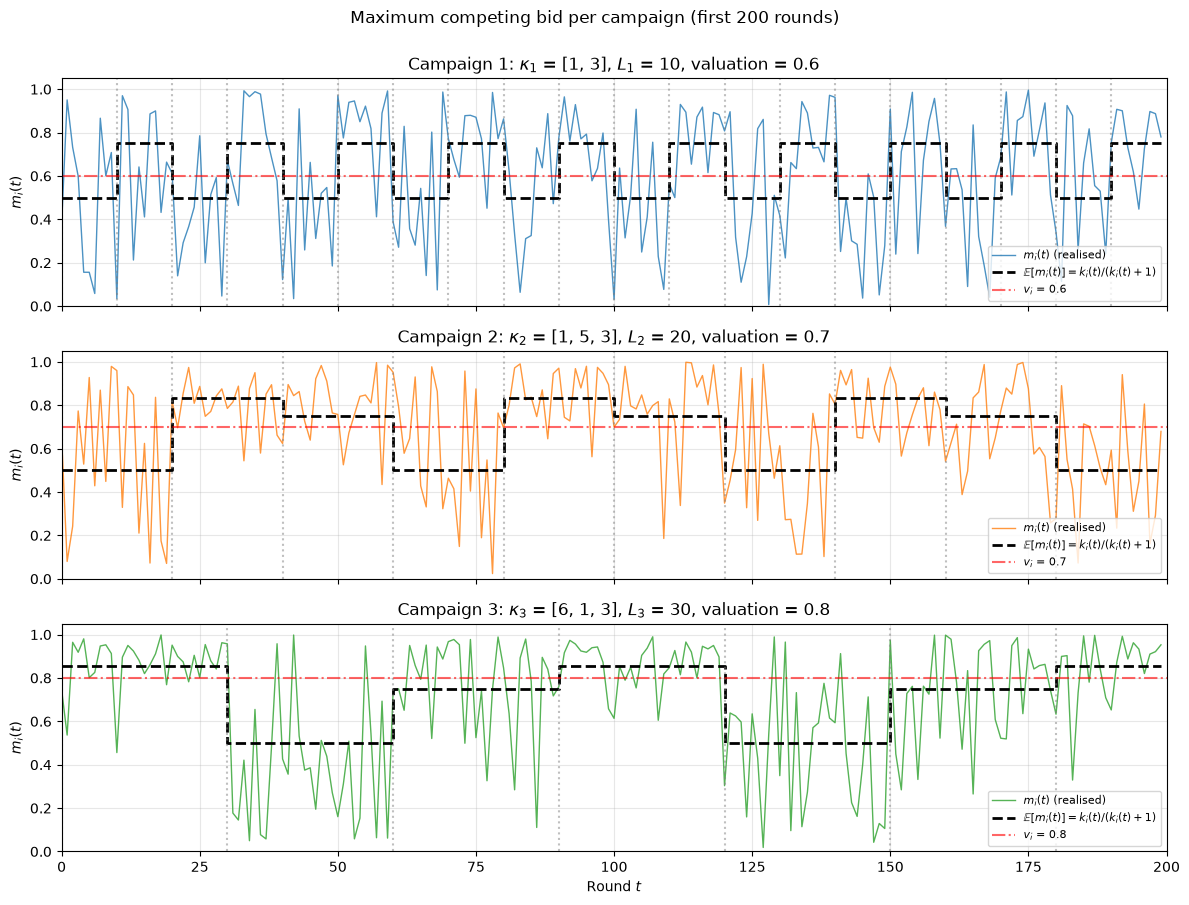
\includegraphics[width=\linewidth,height=0.56\textheight,keepaspectratio]{r3_m_nonstat.png}\\[0.05cm]
    {\tiny Realised $m_i(t)$ with regime mean and valuation $v_i$.}
  \end{column}
\end{columns}
\end{frame}

% - - - - - - - - - - - - - - - - - - - -
\begin{frame}{R3 --- Algorithm: primal-dual pacing over super-arms}
\scriptsize
\textbf{Idea.} An action is a super-arm $a=(S,b)$. Full feedback gives
$f_t(a),\,c_t(a)$ for \emph{every} super-arm, so the primal is an expert problem:
Hedge maximises $L_t(a,\lambda)=f_t(a)-\lambda(c_t(a)-\rho)$ while OGD learns
$\lambda\in[0,1/\rho]$; stop bidding once $B<1$.

\begin{algobox}
\begin{algorithm}[H]
  \scriptsize
  \caption{\scriptsize Primal-dual bidding (full feedback)}
  \KwIn{$B$, $T$, super-arms $\mathcal A$, rates $\eta_p,\eta_d$}
  $\rho\leftarrow B/T$;\; $\lambda_1\leftarrow0$;\; $w_1(a)\leftarrow1$ for all $a$\;
  \For{$t=1,\dots,T$}{
    sample $a_t\sim\gamma_t\propto w_t$; bid $b_t$ on $S_t$; observe wins and $m(t)$\;
    collect $f_t(a_t)$, pay $c_t(a_t)$; $B\leftarrow B-c_t(a_t)$\;
    compute $f_t(a),\,c_t(a)$ for all $a$ from $m(t)$\;
    $w_{t+1}(a)\leftarrow w_t(a)\exp\!\left(\eta_p\,[\,f_t(a)-\lambda_t(c_t(a)-\rho)\,]\right)$\;
    $\lambda_{t+1}\leftarrow\Pi_{[0,\,1/\rho]}\!\left(\lambda_t-\eta_d(\rho-c_t(a_t))\right)$\;
    \If{$B<1$}{play $(\emptyset,\emptyset)$ for the remaining rounds\;}
  }
\end{algorithm}
\end{algobox}
\end{frame}

% - - - - - - - - - - - - - - - - - - - -
\begin{frame}{R3 --- Why it works in both worlds}
\footnotesize
\begin{columns}[T]
  \begin{column}{0.52\textwidth}
    \begin{itemize}
      \item \textbf{No stale averages:} Hedge re-evaluates every super-arm each round from
            the current $m(t)$; $\lambda_t$ prices the budget and makes the primal
            shift to cheaper actions when spending exceeds $\rho$.
      \item \textbf{Same agent, same hyper-parameters} on the stochastic (R2) and the
            highly non-stationary sequence:
            $\eta_p$ on rescaled $L_t$ $=20$, $\eta_d=0.05$, $\lambda_1=0$.
      \item The analysis never uses how $m(t)$ is generated $\Rightarrow$
            sublinear regret in \emph{both} environments:
            $R_{2000}\approx 6$ (stationary) and $\approx 11$ (non-stationary).
      \item \textbf{Guarantee:} regret $O(\sqrt T)$ against the hindsight $\OPT$ and
            $O(\sqrt T)$ budget violation (made exact by the stopping rule).
    \end{itemize}
    \vspace{0.2cm}
    Best of both worlds: stochastic guarantees of UCB-type methods
    \emph{and} adversarial robustness of no-regret learners, with one algorithm.
  \end{column}
  \begin{column}{0.45\textwidth}
    \centering
    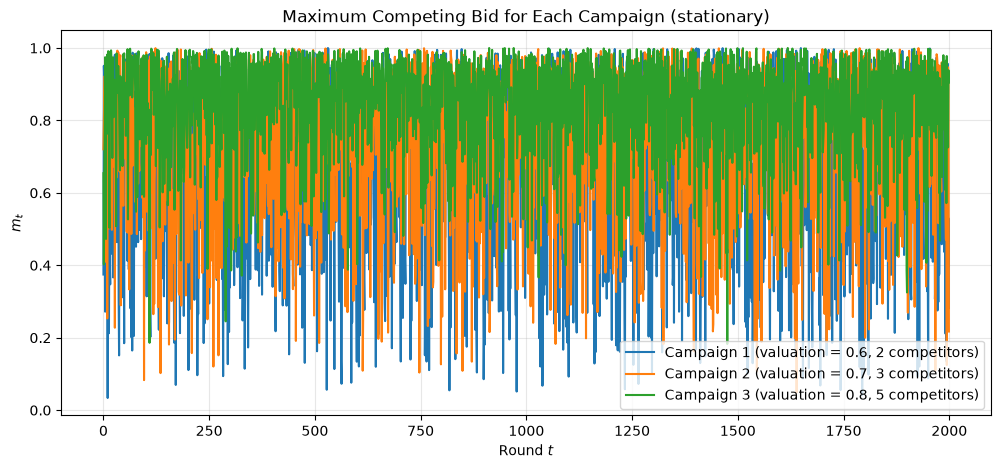
\includegraphics[width=\linewidth,height=0.48\textheight,keepaspectratio]{r3_env_stationary.png}\\[0.1cm]
    {\tiny Stationary sequence (R2 environment): $m_i(t)\sim\mathrm{Beta}(k_i,1)$, $k=(2,3,5)$.}
  \end{column}
\end{columns}
\end{frame}

\begin{frame}{R3 --- Results}
\footnotesize
\centering
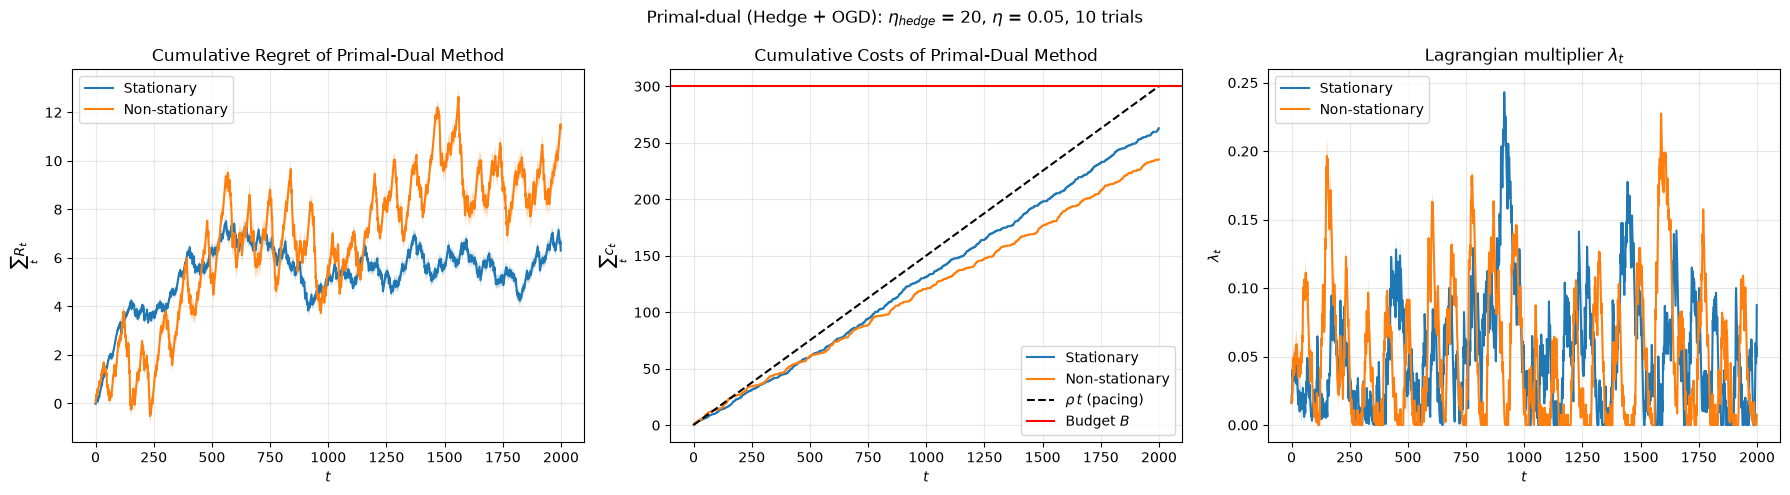
\includegraphics[width=0.94\textwidth,height=0.55\textheight,keepaspectratio]{r3_results.png}\\[0.12cm]
\begin{columns}[T]
  \begin{column}{0.5\textwidth}
    \centering
    \textbf{Stationary:}\\
    regret $6.3\pm0.8$ \quad ($T\cdot\OPT = 121.8$)\\
    spent $262.8/300$
  \end{column}
  \begin{column}{0.5\textwidth}
    \centering
    \textbf{Non-stationary:}\\
    regret $11.3\pm1.5$ \quad ($T\cdot\OPT = 228.7$)\\
    spent $235.2/300$
  \end{column}
\end{columns}
\end{frame}

\begin{frame}{R3 --- Results: learned policy vs clairvoyant}
\footnotesize
\centering
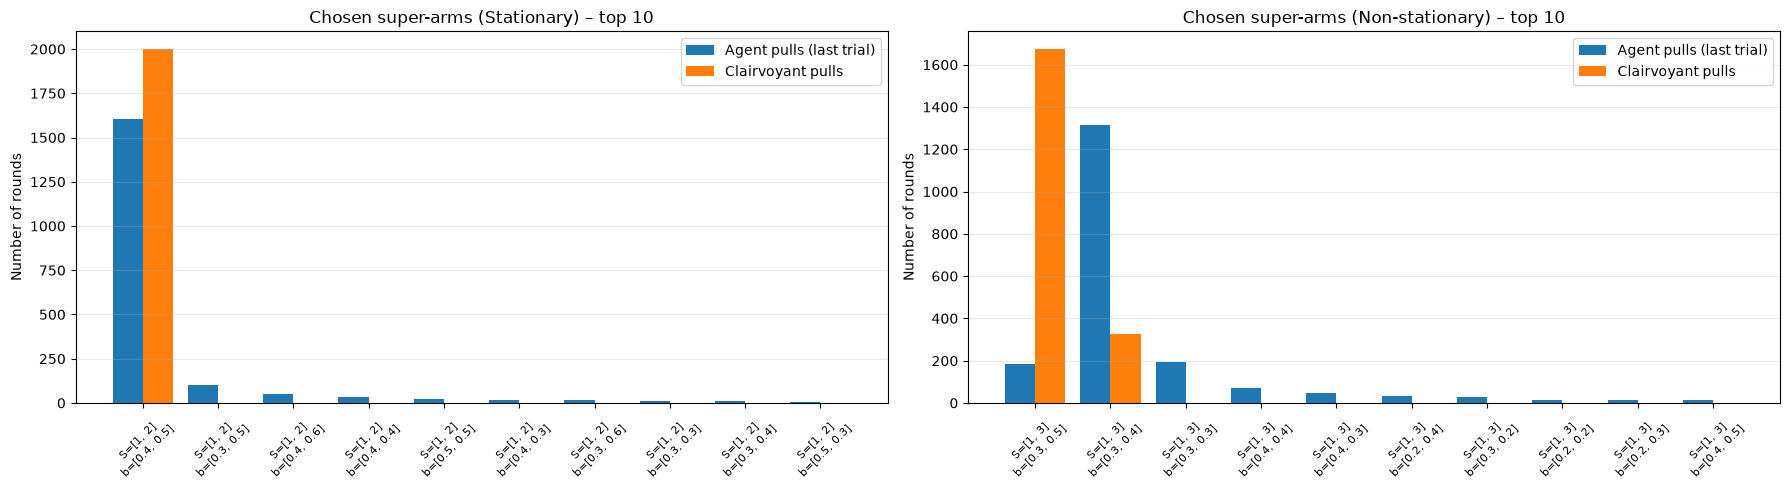
\includegraphics[width=0.94\textwidth,height=0.55\textheight,keepaspectratio]{r3_superarms.png}\\[0.12cm]
\begin{itemize}
  \item \textbf{Stationary:} the agent converges to the clairvoyant super-arm
        ($S=\{1,2\}$, $b=(0.4,0.5)$) in $\sim\!1600$ of $2000$ rounds.
  \item \textbf{Non-stationary:} clairvoyant mixes $b_3\in\{0.4,0.5\}$ on $S=\{1,3\}$;
        agent favours the slightly cheaper $(0.3,0.4)$ --- expected, since $\lambda_t>0$
        penalises cost.
\end{itemize}
\end{frame}

% ####################################################################
\section{Requirement 4 --- Non-stationary environment}
% ####################################################################


\begin{frame}{R4 --- Environment setting}

Non-stationary environment with the following setting:

\begin{itemize}
    \item Slight variations (i.e. not too frequent)
    \item Kept the same mean for highest competing bid for a few hundred iterations
    \item Same highest competing bid across trials (so only variation is randomness within UCB).
\end{itemize}

\end{frame}

% - - - - - - - - - - - - - - - - - - - -
\begin{frame}{R4 --- Algorithm: }

  \begin{algobox}
  \begin{algorithm}[H]
    \scriptsize
    \caption{\scriptsize Combinatorial UCB with Sliding Window}
    \KwIn{... window size ${W}$ ...}
    \For{$t = 1,\dots,T$}{
        % On \texttt{update()}:\;
        % \KwIn{played arms, reward, cost}\;
        % Record "empty" entry for non-played arms\;
        % \If{$t \gt W$}{
        %     \If{$history(t-W) not empty$}{
        %         
        %     }
        % }
      \ForEach{$b \in \bidset$}{
        $\overline{f}_t(b)\leftarrow\frac{1}{N_{W, t-1}(b)}\Sigma_{t'=max(1, t-W)}^{t'=t}f_{t'}(b)\mathbb{I}(b_{t'}=b)$\;
        $\overline{f}_t^{UCB}(b)\leftarrow\overline{f}_t(b)+\sqrt{\frac{2\log(T)}{N_{W, t-1}(b)}}$\;
        $\overline{c}_t(b)\leftarrow\frac{1}{N_{W, t-1}(b)}\Sigma_{t'=max(1, t-W)}^{t'=t}c_{t'}(b)\mathbb{I}(b_{t'}=b)$\;
        $\overline{c}_t^{UCB}(b)\leftarrow\overline{c}_t(b)-\sqrt{\frac{2\log(T)}{N_{W, t-1}(b)}}$\;
      }
      Compute $\gamma_t$ solution of the LP defining $OPT_{t}$ \;
      
      Bid $b_t \sim \gamma_t$ \;
      Observe $f_t(b_t)$ and $c_t(b_t)$\;
      $B\leftarrow B-c_t(b_t)$\;
      \If{$B<1$} {
        Terminate\;
      }
    }
  \end{algorithm}
  \end{algobox}

\end{frame}

% - - - - - - - - - - - - - - - - - - - -
\begin{frame}{R4 --- Algorithm }

  \begin{algobox}
  \begin{algorithm}[H]
    \scriptsize
    \caption{\scriptsize Combinatorial UCB with Change Detection}
    \KwIn{... change ${\epsilon}$, change detection threshold ${h}$ ...}
    $\tau_b \leftarrow 1$ for all $b\in\bidset$ \tcp*{last detected change per arm}

    \For{$t = 1,\dots,T$}{
      \ForEach{$b \in \bidset$}{
        $\overline{f}_t(b)\leftarrow\frac{1}{N_{\tau_b, t-1}(b)}\Sigma_{t'=\tau_b}^{t'=t}f_{t'}(b)\mathbb{I}(b_{t'}=b)$\;
        $\overline{f}_t^{UCB}(b)\leftarrow\overline{f}_t(b)+\sqrt{\frac{2\log(T)}{N_{\tau_b, t-1}(b)}}$\;
        $\overline{c}_t(b)\leftarrow\frac{1}{N_{\tau_b, t-1}(b)}\Sigma_{t'=\tau_b}^{t'=t}c_{t'}(b)\mathbb{I}(b_{t'}=b)$\;
        $\overline{c}_t^{UCB}(b)\leftarrow\overline{c}_t(b)-\sqrt{\frac{2\log(T)}{N_{\tau_b, t-1}(b)}}$\;
      }

     Same as other Combinatorial UCB... \;

     \If{\texttt{change-detected}($f_t(b_t), c_t(b_t)$)}{
        $\tau_b \leftarrow t$ \;
     }
      
      $B\leftarrow B-c_t(b_t)$ ...\;
    }
  \end{algorithm}
  \end{algobox}


\end{frame}

\begin{frame}{R4 --- Results: Sliding Window}

\centering
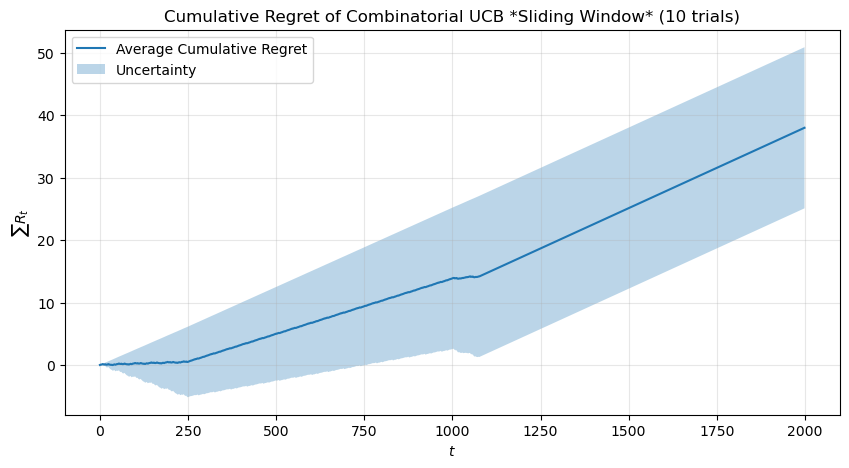
\includegraphics[width=0.48\textwidth,keepaspectratio]{r4_sliding_window_regret.png}\hfill
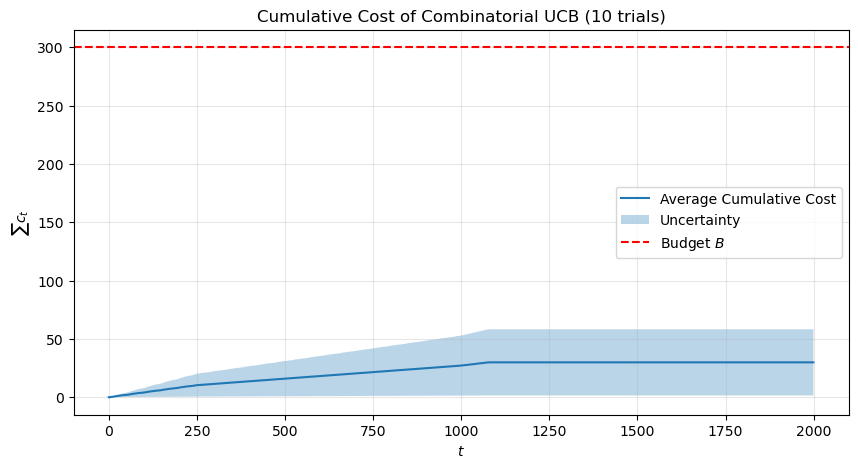
\includegraphics[width=0.48\textwidth,keepaspectratio]{r4_sliding_window_cost.png}


\end{frame}


\begin{frame}{R4 --- Results: Change Detection}

\centering
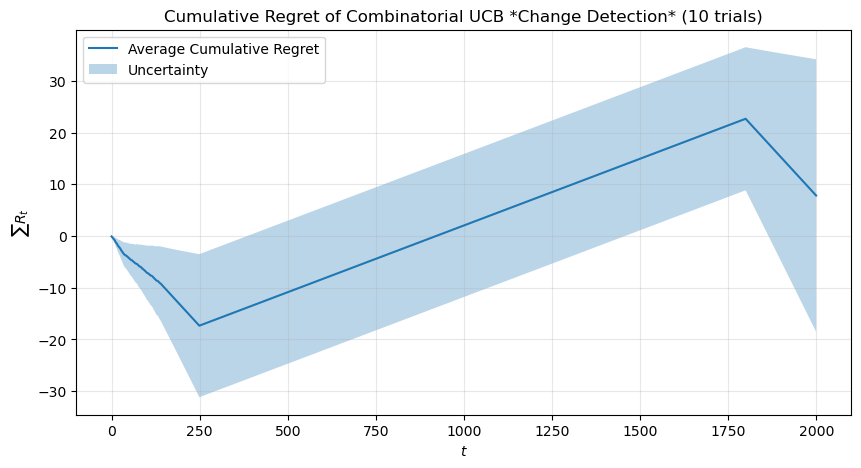
\includegraphics[width=0.48\textwidth,keepaspectratio]{r4_change_detection_regret.png}\hfill
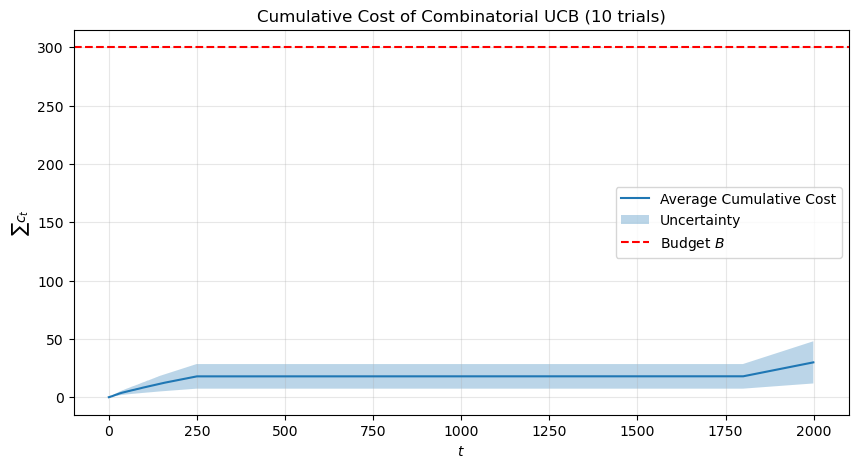
\includegraphics[width=0.48\textwidth,keepaspectratio]{r4_change_detection_cost.png}



\end{frame}

% ####################################################################
\section{Discussion \& Conclusion}
% ####################################################################

\begin{frame}{Discussion}
\scriptsize
\begin{itemize}
  \item \textbf{Stochastic (R1, R2): UCB-like methods learn the right arms} but the regret still grows
        almost linearly over our horizon. Two reasons: the gaps between the best bids are tiny
        ($10^{-4}$--$10^{-3}$), and the LCB on the cost makes the LP mis-pace the spend:
        in R1 the budget is never binding ($85/300$), in R2 it is exhausted $\sim\!300$ rounds early.
  \item \textbf{Combinatorial structure pays off.} Estimating base arms $(i,b)$ and summing them
        is what makes $102$ super-arms tractable; the conflict graph is handled for free by
        restricting the LP to feasible super-arms.
  \item \textbf{Primal-dual (R3) is the most robust.} With one set of hyper-parameters it reaches
        regret $\approx 6$ (stationary) and $\approx 11$ (non-stationary) at $T=2000$ and spends
        $80$--$90\%$ of the budget: the dual variable $\lambda_t$ prices the budget and paces the
        spend over the whole horizon.
  \item \textbf{Non-stationarity (R4).} Sliding window and change detection both recover after a
        regime change, but they trade adaptivity for variance: a short window forgets useful data,
        a long one reacts late.
  \item \textbf{Limitations.} Small instances ($N=3$, $|\bidset|\le 11$), i.i.d.\ uniform competitors,
        fixed valuations, and only one seed for the R3 adversarial sequence.
\end{itemize}
\end{frame}

\begin{frame}{Conclusions}
\scriptsize
\begin{itemize}
  \item We modelled multi-campaign bidding in first-price auctions as a \emph{budgeted combinatorial
        bandit} with a conflict graph, and built the clairvoyant benchmarks as linear programs.
  \item \textbf{R1:} UCB1 and its budgeted extension converge to the optimal bid $0.4$.
  \item \textbf{R2:} Combinatorial-UCB with base-arm estimates respects the budget and the conflict
        graph, with sublinear-looking regret dominated by near-equivalent super-arms.
  \item \textbf{R3:} A single primal-dual learner works in both the stochastic and the adversarial
        world, with the lowest regret of all methods tested.
  \item \textbf{R4:} Sliding-window and change-detection variants of Combinatorial-UCB handle
        slowly-varying competitors; the primal-dual method remains a strong baseline.
\end{itemize}
\vspace{0.2cm}
\textbf{Future work:} tune the confidence radius (e.g.\ Bernstein bounds) to improve
budget pacing, learn the conflict structure online, and scale to more campaigns via
LP relaxations instead of enumerating super-arms.
\end{frame}

\begin{frame}[plain,c]
  \centering
  {\Huge Thank you!}
\end{frame}


% ####################################################################
\appendix
% ####################################################################

\begin{frame}{Appendix --- R1 budget consumption}
\scriptsize
\begin{columns}[T]
  \begin{column}{0.5\textwidth}
    \centering
    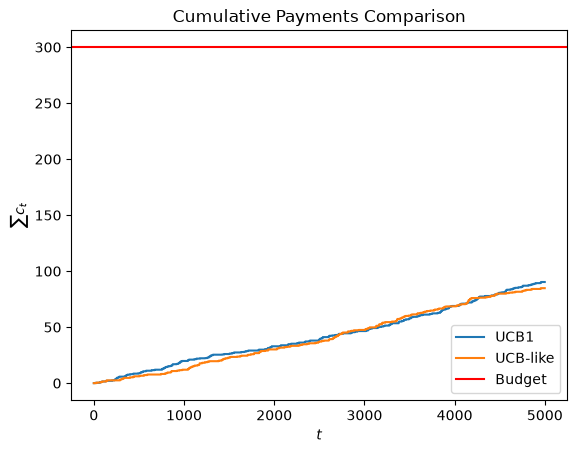
\includegraphics[width=\linewidth,height=0.52\textheight,keepaspectratio]{r1_payments_comparison.png}\\[0.03cm]
    {\tiny Cumulative payments of UCB1 vs.\ the budgeted UCB-like agent (single run).}
  \end{column}
  \begin{column}{0.5\textwidth}
    \centering
    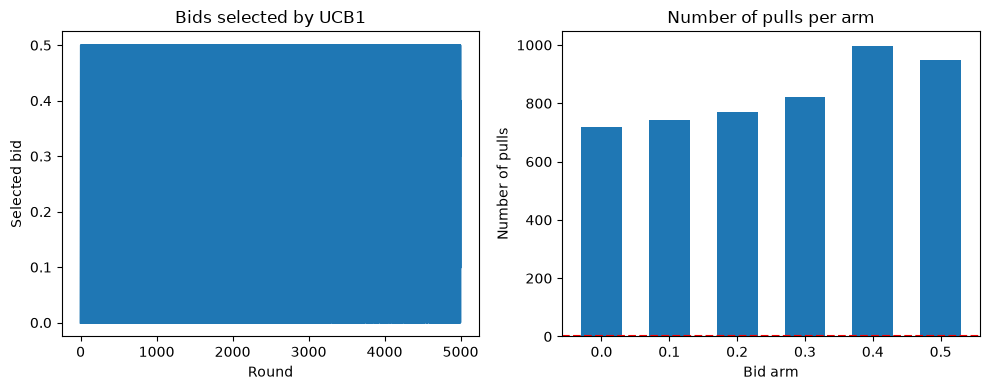
\includegraphics[width=\linewidth,height=0.52\textheight,keepaspectratio]{r1_ucb1_bids.png}\\[0.03cm]
    {\tiny Bids chosen by UCB1 over time and number of pulls per arm.}
  \end{column}
\end{columns}
\vspace{0.1cm}
With $\rho=0.06$ and an optimal per-round cost of $0.026$, the budget of $300$ is far from binding:
only $\approx 85$ is spent in $5000$ rounds, so the budgeted and unbudgeted learners behave the same.
\end{frame}



\end{document}
